\subsection{Т1}

\textbf{Задание:}
Случайная величина распределенна равномерно на отрезке [0, $\theta$]. по выборке обьема n найденны оценки \\
параметра 
\begin{equation*}
    \theta : \tilde\theta_1 = 2\overline{x}, \; 
             \tilde\theta_2 = x_{min} \;
             \tilde\theta_3 = x_{max} \;
             \tilde\theta_4 = x_{min} + x_{min} \;
             \tilde\theta_5 = \Bigg(x_1 + \frac{\sum\limits_{k=2}^n x_k}{(n-1)}\Bigg). 
\end{equation*}
\noindent

% \paragraph{Пункт "а"}

\subsubsection{Пункт <<a>>}
\vspace{1.5mm}
\textbf{1:} 
$\tilde\theta_1 = 2\overline{x}$ \\
\begin{equation*}
    M_{\tilde\theta_1} = M\left[ \frac{2}{n} \sum{x_i}\right] 
    = \frac{2}{n} \sum  M_{x_i} = \frac{2}{n} \:n\: \frac{\theta}{2} = \theta
\end{equation*}
$\Rightarrow$ \textbf{несмещённая}

\begin{equation*}
    D_{\tilde\theta_1} = D\left[ \frac{4}{n^2} \sum{x_i}\right] 
    = \frac{2}{n} \sum  D_{x_i} = \frac{4}{n^2} \:n\: D_{\xi} 
    = \left( \xi \thicksim \; R(a,b) \hspace{2.5 mm} D_{\xi} = \frac{(b-a)^2}{12}\right) =
\end{equation*}

\begin{equation*}
    = \frac{4}{n} \; \frac{\theta^2}{12} = \frac{\theta^2}{3n} \to 0 \; (n \to \infty)
\end{equation*}
$\Rightarrow$ \textbf{состоятельная}
\vspace{1.5 mm} \\
\begin{center}
    \textbf{не смещённая} $\Rightarrow$ \textbf{ассимптотически несмещённая}
\end{center}

\vspace{2.5 mm}
\textbf{2:}
$\tilde\theta_2 = x_{min}$
\begin{equation*}
    M\left[ \tilde\theta_2 \right] = M\left[ x_{min} \right]
\end{equation*}
\begin{equation*}
    \varphi(y) = n\left(1-F(y)  \right)^{n-1} p(y) = n\left(1 - \frac{y}{\theta}\right)^{n-1}\frac{1}{\theta}(0;\theta)
\end{equation*}
\begin{equation*}
    M_{x_{min}} = \int_{0}^{\theta}n\left[\left(1 - \frac{y}{\theta}\right)^{n-1}\frac{1}{\theta}\right]\,\mathrm{d}y =
\end{equation*}
\begin{center}
    Замена $ t = \frac{y}{\theta}$ 
\end{center}
\begin{equation*}
    = \int_{0}^{1}\theta tn(1 - t)^{n-1}\,\mathrm{d}t = n\theta B(2,n) = n\theta \frac{\Gamma(n)\Gamma(2)}{\Gamma(n+2)} = \frac{\theta}{n+1} 
\end{equation*} 
$\Rightarrow$ \textbf{смещённая} \\
\vspace{1.5mm}\\
\begin{flushleft}
    
\includegraphics[width=0.04\textwidth]{images/present.png} 
    \textbf{Подарок: <<Ассимптотическая несмещённость исходной оценки>>}
\end{flushleft}
\begin{equation*}
    M_{x_{min}} = \frac{\theta}{n+1} = \to 0 \;\;(n\to\infty)
\end{equation*}
$\Rightarrow$ \textbf{асимптотически не смещённая} \\
\vspace{1.5mm}\\
Возьмем новую оценку $\tilde{\theta_2}' = (n+1)\tilde\theta_2$, которая будет несмещённой.
\vspace{2.5 mm}\\
\begin{equation*}
    D\left[\tilde{\theta_2}' \right] = M\left[\tilde{\theta_2}'^2 \right] - M^2\left[\tilde{\theta_2}' \right]
\end{equation*}
\begin{equation*}
    M\left[\tilde{\theta_2}'^2 \right] = \int_{0}^{\theta}y^2\left[ n\left(1-\frac{y}{\theta}\right)\right]\,\mathrm{d}y = 
    \int_{0}^{1}y^2 \theta^2nt^2\left(1-t\right)^{n-1}\,\mathrm{d}y = \theta^2n B(3, n) = n\theta^2\frac{\Gamma(3)\Gamma(n)}{\Gamma(n+3)} =
\end{equation*}
\vspace{1.5 mm}
\begin{equation*}
    = n\theta^2\frac{\Gamma(3)\Gamma(n)}{(n+2)(n+2)n\Gamma(n)} = \frac{2\theta^2}{(n+2)(n+1)}
\end{equation*}
\vspace{1.5 mm}
\begin{equation*}
    D\left[x_{min} \right] = \frac{2\theta^2}{(n+2)(n+1)} - \frac{\theta^2}{(n+1)^2} = \frac{\theta^2}{(n+1)^2(n-2)}
\end{equation*}
\vspace{1.5 mm}
\begin{equation*}
    D\left[\tilde{\theta_2}' \right]  = \frac{n\theta^2}{(n-1)(n+2)}
\end{equation*}
\vspace{1.5 mm}
Теперь посмотрим на состоятельность $\tilde{\theta_2}'$
\begin{equation*}
    \forall\varepsilon > 0 \; \mathcal{P}\left(|\tilde{\theta_2}' - \theta| \geqslant \varepsilon\right) \to 0\;\;(n\to\infty)
\end{equation*}
\vspace{1.5 mm}
\begin{equation*}
    \mathcal{P}\left(|\tilde{\theta_2}' - \theta| \geqslant \varepsilon\right) \geqslant \mathcal{P}\left(\tilde{\theta_2}' \geqslant \theta+\varepsilon\right)
    =  \mathcal{P}\left(x_{min}\geqslant \frac{\theta+\varepsilon}{n+1}\right) 
    =  \mathcal{P}\left(x_{1}\geqslant \frac{\theta+\varepsilon}{n+1}, x_{2}\geqslant \frac{\theta+\varepsilon}{n+1}, \;\dotsi,\; x_{n}\geqslant \frac{\theta+\varepsilon}{n+1} \right)
    =
\end{equation*}
\vspace{1.5 mm}
\begin{equation*}
    = \prod\limits_{i=1}^n\;\mathcal{P}\left(x_{i}\geqslant \frac{\theta+\varepsilon}{n+1}\right) 
    = \prod\limits_{i=1}^n\;\Bigg(1 - \mathcal{P}\left(x_{i} < \frac{\theta+\varepsilon}{n+1}\right)\Bigg)
    = \Bigg(1 - \digamma\left(\frac{\theta+\varepsilon}{n+1}\right)\Bigg)^n
    = \Bigg(1 - \frac{\theta+\varepsilon}{n+1}\Bigg)^n
    \to e^{-\frac{\theta+\varepsilon}{\theta}} > 0  
\end{equation*} 
\vspace{1.5mm}
\textbf{не стремится к 0 => не состоятельная}
\vspace{1.5mm}\\
\begin{flushleft}
    
\includegraphics[width=0.04\textwidth]{images/present.png} 
    \textbf{Подарок: <<Состоятельность неисправленной оценки>>}
\end{flushleft}
\begin{equation*}
    D\left[x_{min} \right] = \frac{\theta^2}{(n+1)^2(n-2)} \to 0 \;\; (n\to\infty)
\end{equation*}
$\Rightarrow$ \textbf{состоятельная} \\
\vspace{2.5mm}
\begin{flushleft}
    
\includegraphics[width=0.04\textwidth]{images/present.png} 
    \textbf{Подарок: <<Предельный закон распределения>>}
\end{flushleft}
\vspace{2.5mm}

\textbf{3:} 
$\tilde\theta_3 = x_{max}$
\begin{equation*}
    x_i\thicksim\digamma(x) \hspace{4mm} x_{max} \thicksim \Big(\digamma(y)\Big)^n \hspace{4mm} 
    p(y)_{x_{max}} = n\Big(\digamma(y)\Big)^{n-1}p(y)\;\left(0;\theta\right)
\end{equation*}
\begin{equation*}
    M\left[\tilde\theta_3\right] = \int_{0}^{\theta}ny\left[\left(\frac{y}{\theta}\right)^{n-1}\frac{1}{\theta}\right]\,\mathrm{d}y
    = \frac{n}{\theta^{n}}\int_{0}^{\theta}y^n\,\mathrm{d}y
    = \frac{n\theta}{n+1}
\end{equation*}
 \textbf{смещённая, $\Rightarrow$ ассимтотически не смещённая}\\
Рассмотрим новую оценку $\tilde{\theta_3}' = \frac{n+1}{n}x_{max}$, которая будет несмещённой.\\
\begin{equation*}
    M\left[\tilde{\theta_3}^2\right] = \int_{0}^{\theta}ny^2\left[\left(\frac{y}{\theta}\right)^{n-1}\frac{1}{\theta}\right]\,\mathrm{d}y
    = \frac{n}{\theta^{n}}\int_{0}^{\theta}y^{n+1}\,\mathrm{d}y
    = \frac{n\theta^2}{n+2}
\end{equation*}
\vspace{2.5mm}
\begin{equation*}
    D\left[\tilde{\theta_3}\right] = \frac{n\theta^2}{n+2} - \frac{(n\theta)^2}{(n+1)^2} = \frac{\theta^2n}{(n+2)(n+1)^2}
\end{equation*}
\vspace{1.5mm}
\begin{equation*}
    D\left[\tilde{\theta_3}'\right] = \frac{(n+1)^2}{n^2}\frac{\theta^2n}{(n+2)(n+1)^2}
    = \frac{\theta^2}{n(n+2)} \to 0 \;\; (n \to \infty)
\end{equation*}\\
$\Rightarrow$ \textbf{состоятельная по достаточному условию}\\
\vspace{1.5mm}\\
\begin{flushleft}
    
\includegraphics[width=0.04\textwidth]{images/present.png} 
    \textbf{Подарок: <<Состоятельность неисправленной оценки>>}
\end{flushleft}
\begin{equation*}
   D\left[x_{max} \right] =  \frac{\theta^2n}{(n+2)(n+1)^2} \to 0 \;\; (n\to\infty)
\end{equation*}
$\Rightarrow$ \textbf{состоятельная} \\

\textbf{4:}
$\tilde\theta_4 = x_{min} + x_{max}$
\begin{equation*}
    M\left[\tilde{\theta_4}\right] = M\left[x_{min}\right] + M\left[x_{max}\right]
    = \frac{n\theta}{n+1} + \frac{\theta}{n+1} = \theta
\end{equation*}
$\Rightarrow$ \textbf{не смещённая}\\
\begin{equation*}
    D\left[\tilde{\theta_4}\right] = D\left[x_{min}\right] + D\left[x_{max}\right] + 2cov(x_{min}, x_{max})
\end{equation*}
\vspace{1.5mm}
\begin{equation*}
    cov(x_{min}, x_{max}) =  M\left[x_{min}*x_{max}\right] -M\left[x_{min}\right] * M\left[x_{max}\right]
\end{equation*}
\vspace{1.5mm}
\begin{equation*}
    p(y;z) = n(n-1)(\digamma(z) - \digamma(y))^{n-2}p(z)p(y) \;\; (z \geqslant y )
\end{equation*}
\vspace{1.5mm}
\begin{equation*}
    M\left[x_{min}*x_{max}\right] = \varoiint_{D}yzn(n-1)\left(\frac{z}{\theta} - \frac{y}{\theta}\right)^{n-2}\theta^{-2} \,\mathrm{d}z\mathrm{d}y
    = \int_{0}^{\theta}\mathrm{d}z\int_{0}^{z}yzn(n-1)\left(\frac{z}{\theta} - \frac{y}{\theta}\right)^{n-2}\theta^{-2}\mathrm{d}y =
\end{equation*}
\vspace{1.5mm}
\begin{center}
    Замена t = $\frac{y}{z}$
\end{center}
\vspace{1.5mm}
\begin{equation*}  
    = \frac{n(n-1)}{\theta^n}\int_{0}^{\theta}\mathrm{d}z\int_{0}^{1}tz^3\left(z-tz\right)^{n-2}\mathrm{d}y
    = \frac{n(n-1)}{\theta^n}\int_{0}^{\theta}z^{n+1}\mathrm{d}z\int_{0}^{1}t\left(1-t\right)^{n-2}\mathrm{d}y
    = B(2, n-1)\;\frac{n(n-1)}{\theta^n}\int_{0}^{\theta}z^{n+1}\mathrm{d}z
\end{equation*}
\vspace{1.5mm}
\begin{equation*}  
    B(2, n-1) = \frac{\Gamma(2)\Gamma(n-1)}{\Gamma(n+1)} = \frac{\Gamma(2)\Gamma(n-1)}{n\Gamma(n)} = \frac{(n-2)!}{n!}  = \frac{1}{n(n-1)}
\end{equation*}
\vspace{1.5mm}
\begin{equation*}  
    M\left[x_{min}*x_{max}\right]  = \frac{1}{\theta^n}\int_{0}^{\theta}z^{n+1}\mathrm{d}z
    = \frac{\theta^2}{n+2}
\end{equation*}
\vspace{1.5mm}
\begin{equation*}  
    cov(x_{min}, x_{max}) = \frac{\theta^2}{n+2} - \frac{\theta}{n+1}\frac{\theta n}{n+1} = \frac{\theta^2}{(n+2)(n+1)^2}
\end{equation*}
\vspace{1.5mm}
\begin{equation*}  
    D\left[\tilde{\theta_4}\right] =\frac{\theta^2n}{(n+2)(n+1)^2} +2\frac{\theta^2n}{(n+2)(n+1)^2} +2\frac{\theta^2}{(n+2)(n+1)^2}
    = \frac{2\theta^2}{(n+2)(n+1)} \to 0 \;\;\left(n\to\infty\right)
\end{equation*}
\vspace{1.5mm}
$\Rightarrow$ \textbf{состоятельная по достаточному условию}\\
\vspace{2.5mm}\\
\begin{flushleft}
    
\includegraphics[width=0.04\textwidth]{images/present.png} 
    \textbf{Подарок: <<Ассимптотическая нормальность оценки>>}
\end{flushleft}
\begin{equation*}
   \eta = \sqrt{n}\left(x_{min}(n+1) - \theta\right) \rightsquigarrow
\end{equation*}
% Функция распределения размаха выборки может быть найдена следующим образом:

% Пусть $F_{\min}(x)$ и $F_{\max}(x)$ - функции распределения минимума и максимума соответственно. Тогда вероятность того, что размах выборки будет меньше или равен $x$, равна вероятности того, что минимум выборки будет меньше или равен $y$ и максимум выборки будет больше или равен $y+x$, где $y$ - произвольное число. Таким образом, функция распределения размаха выборки может быть записана как:

% $$
% F_{\text{размах}}(x) = P(\max(X_1, X_2, ..., X_n) - \min(X_1, X_2, ..., X_n) \leq x) \\
% = \int_{-\infty}^{\infty} P(\min(X_1, X_2, ..., X_n) \leq y)P(\max(X_1, X_2, ..., X_n) \geq y+x) dy \\
% = \int_{-\infty}^{\infty} [1-F_{\min}(y)]F_{\max}(y+x)dy
% $$

% Таким образом, функция распределения размаха выборки может быть найдена путем интегрирования произведения функций распределения минимума и максимума.
\textbf{5:}
$\tilde\theta_5 = \Big(x_1 + \frac{\sum\limits_{k=2}^n x_k}{(n-1)}\Big)$
\begin{equation*}
    M\left[\tilde{\theta_5}\right] = M[x_1] + \frac{n-1}{n-1}M[x_2] = \theta
\end{equation*}
$\Rightarrow$ \textbf{не смещённая}
\vspace{1.5 mm} \\
\begin{center}
    \textbf{не смещённая} $\Rightarrow$ \textbf{ассимптотически несмещённая}
\end{center}
\vspace{1.5mm}
\begin{equation*}  
    D\left[\tilde{\theta_5}\right] = D[x_1] + \frac{n-1}{(n-1)^2}D[x_2]
    = \frac{\theta^2}{12}\left(1 + \frac{1}{n-1}\right) \nrightarrow 0 \;\;(n\to\infty)
\end{equation*}
\vspace{1.5mm}
\begin{center}
    Достаточное условие не работает!!!
\end{center}
\vspace{1.5mm}
\begin{equation*}
    x_1 + \frac{\sum\limits_{k=2}^n x_k}{(n-1)}
    \xrightarrow[]{\mathcal{P}} x_1 + \frac{\theta}{2}
\end{equation*}
$\Rightarrow$ \textbf{не является состоятельной}


\newpage
\vspace{1cm}
\subsubsection{Пункт <<б>>}

Полученные графики для оценок для случайно сгенерированой выборки из N=100 элементов
\begin{center}
    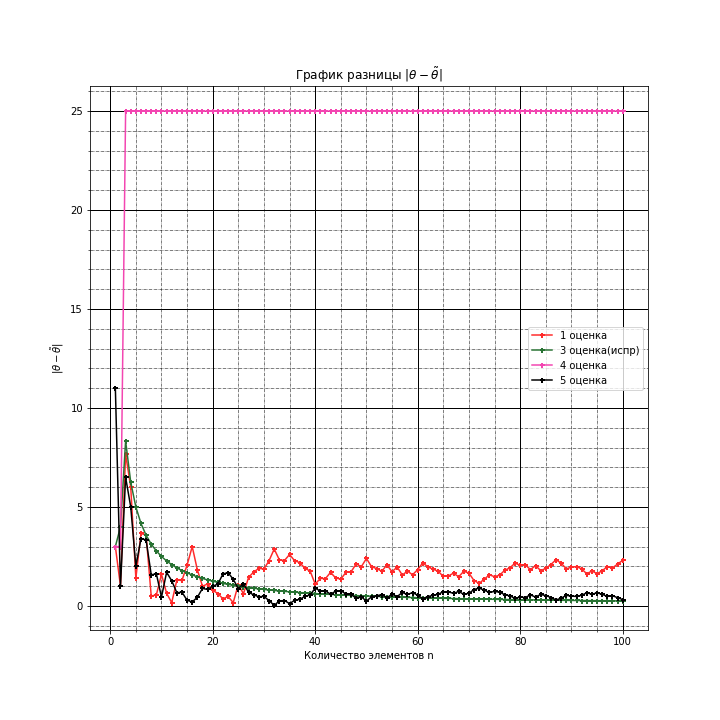
\includegraphics[width=1.1\textwidth]{images/ex_1/1.png}
    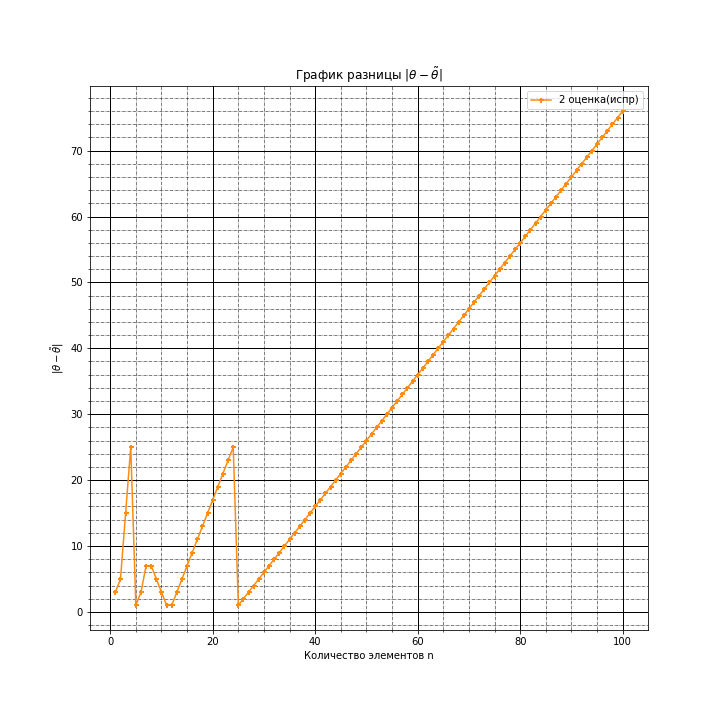
\includegraphics[width=1.1\textwidth]{images/ex_1/2.png}
\end{center}
% \pagebreak
\newpage